%%%%%%%%%%%%%%%%%%%%%%%%%%%%%%%%%%%%%%%%%%%%%%%%%%%%%%%%%%%%%%%%%%%%%%
%DIF LATEXDIFF DIFFERENCE FILE
%DIF DEL ../masterThesis_old/diss.tex   Fri Jul 24 12:02:42 2015
%DIF ADD diss.tex                       Wed Jul 22 18:29:03 2015
%%  disstemplate.tex, to be compiled with latex.		     %
%%  08 April 2002	Version 4				     %
%%%%%%%%%%%%%%%%%%%%%%%%%%%%%%%%%%%%%%%%%%%%%%%%%%%%%%%%%%%%%%%%%%%%%%
%%								     %
%%  Writing a Doctoral Dissertation with LaTeX at		     %
%%	the University of Texas at Austin			     %
%%								     %
%%  (Modify this ``template'' for your own dissertation.)	     %
%%								     %
%%%%%%%%%%%%%%%%%%%%%%%%%%%%%%%%%%%%%%%%%%%%%%%%%%%%%%%%%%%%%%%%%%%%%%


\documentclass[12pt]{report}	% The documentclass must be ``report''.

\usepackage{utdiss2}  		% Dissertation package style file.


%%%%%%%%%%%%%%%%%%%%%%%%%%%%%%%%%%%%%%%%%%%%%%%%%%%%%%%%%%%%%%%%%%%%%%
% Optional packages used for this sample dissertation. If you don't  %
% need a capability in your dissertation, feel free to comment out   %
% the package usage command.					     %
%%%%%%%%%%%%%%%%%%%%%%%%%%%%%%%%%%%%%%%%%%%%%%%%%%%%%%%%%%%%%%%%%%%%%%

\usepackage{amsmath,amsthm,amsfonts,amscd} 
				% Some packages to write mathematics.
\usepackage{eucal} 	 	% Euler fonts
\usepackage{verbatim}      	% Allows quoting source with commands.
\usepackage{makeidx}       	% Package to make an index.
\usepackage{url}		% Allows good typesetting of web URLs.
%\usepackage{draftcopy}		% Uncomment this line to have the
				% word, "DRAFT," as a background
				% "watermark" on all of the pages of
				% of your draft versions. When ready
				% to generate your final copy, re-comment
				% it out with a percent sign to remove
				% the word draft before you re-run
				% Makediss for the last time.
\usepackage{latexsym}
\usepackage{natbib}
\usepackage{graphicx}
\usepackage{caption}
\usepackage{subcaption}
\usepackage{listings}
\usepackage{algorithm}
\usepackage{algpseudocode}
\usepackage{amssymb} 
\usepackage{color}
\usepackage{multirow}

\graphicspath{{nips15/}{RLLiterature/}}

\author{Shun Zhang}

\address{9905 Chukar Circle\\ Austin, Texas 78758}  % Required

\title{Parameterized Modular Inverse Reinforcement Learning}
                                                    % Required

%%%%%%%%%%%%%%%%%%%%%%%%%%%%%%%%%%%%%%%%%%%%%%%%%%%%%%%%%%%%%%%%%%%%%%
% NOTICE: The total number of supervisors and other members %%%%%%%%%%
%%%%%%%%%%%%%%% MUST be seven (7) or less! If you put in more, %%%%%%%
%%%%%%%%%%%%%%% they are put on the page after the Committee %%%%%%%%%
%%%%%%%%%%%%%%% Certification of Approved Version page. %%%%%%%%%%%%%%
%%%%%%%%%%%%%%%%%%%%%%%%%%%%%%%%%%%%%%%%%%%%%%%%%%%%%%%%%%%%%%%%%%%%%%

%%%%%%%%%%%%%%%%%%%%%%%%%%%%%%%%%%%%%%%%%%%%%%%%%%%%%%%%%%%%%%%%%%%%%%
%
% Enter names of the supervisor and co-supervisor(s), if any,
% of your dissertation committee. Put one name per line with
% the name in square brackets. The name on the last line, however,
% must be in curly braces.
%
% If you have only one supervisor, the entry below will read:
%
%	\supervisor
%		{Supervisor's Name}
%
% NOTE: Maximum three supervisors. Minimum one supervisor.
% NOTE: The Office of Graduate Studies will accept only two supervisors!
% 
%
\supervisor
	{Prof. Dana Ballard}

%%%%%%%%%%%%%%%%%%%%%%%%%%%%%%%%%%%%%%%%%%%%%%%%%%%%%%%%%%%%%%%%%%%%%%
%
% Enter names of the other (non-supervisor) members(s) of your
% dissertation committee. Put one name per line with the name
% in square brackets. The name on the last line, however, must
% be in curly braces.
%
% NOTE: Maximum six other members. Minimum zero other members.
% NOTE: The Office of Graduate Studies may restrict you to a total
%	of six committee members.
%
%
\committeemembers
	{Prof. Peter Stone}

%%%%%%%%%%%%%%%%%%%%%%%%%%%%%%%%%%%%%%%%%%%%%%%%%%%%%%%%%%%%%%%%%%%%%%

\previousdegrees{B.S.}
     % The abbreviated form of your previous degree(s).
     % E.g., \previousdegrees{B.S., MBA}.
     %
     % The default value is `B.S., M.S.'

%\graduationmonth{...}      
     % Graduation month, either May, August, or December, in the form
     % as `\graduationmonth{May}'. Do not abbreviate.
     %
     % The default value (either May, August, or December) is guessed
     % according to the time of running LaTeX.

%\graduationyear{...}   
     % Graduation year, in the form as `\graduationyear{2001}'.
     % Use a 4 digit (not a 2 digit) number.
     %
     % The default value is guessed according to the time of 
     % running LaTeX.

%\typist{...}       
     % The name(s) of typist(s), put `the author' if you do it yourself.
     % E.g., `\typist{Maryann Hersey and the author}'.
     %
     % The default value is `the author'.


%%%%%%%%%%%%%%%%%%%%%%%%%%%%%%%%%%%%%%%%%%%%%%%%%%%%%%%%%%%%%%%%%%%%%%
% Commands for master's theses and reports.			     %
%%%%%%%%%%%%%%%%%%%%%%%%%%%%%%%%%%%%%%%%%%%%%%%%%%%%%%%%%%%%%%%%%%%%%%
%
% If the degree you're seeking is NOT Doctor of Philosophy, uncomment
% (remove the % in front of) the following two command lines (the ones
% that have the \ as their second character).
%
\degree{MASTER OF SCIENCE}
\degreeabbr{M.S.}

% Uncomment the line below that corresponds to the type of master's
% document you are writing.
%
%\masterreport
\masterthesis


%%%%%%%%%%%%%%%%%%%%%%%%%%%%%%%%%%%%%%%%%%%%%%%%%%%%%%%%%%%%%%%%%%%%%%
% Some optional commands to change the document's defaults.	     %
%%%%%%%%%%%%%%%%%%%%%%%%%%%%%%%%%%%%%%%%%%%%%%%%%%%%%%%%%%%%%%%%%%%%%%
%
%\singlespacing
%\oneandonehalfspacing

%\singlespacequote
\oneandonehalfspacequote

\topmargin 0.125in	% Adjust this value if the PostScript file output
			% of your dissertation has incorrect top and 
			% bottom margins. Print a copy of at least one
			% full page of your dissertation (not the first
			% page of a chapter) and measure the top and
			% bottom margins with a ruler. You must have
			% a top margin of 1.5" and a bottom margin of
			% at least 1.25". The page numbers must be at
			% least 1.00" from the bottom of the page.
			% If the margins are not correct, adjust this
			% value accordingly and re-compile and print again.
			%
			% The default value is 0.125"

		% If you want to adjust other margins, they are in the
		% utdiss2-nn.sty file near the top. If you are using
		% the shell script Makediss on a Unix/Linux system, make
		% your changes in the utdiss2-nn.sty file instead of
		% utdiss2.sty because Makediss will overwrite any changes
		% made to utdiss2.sty.

%%%%%%%%%%%%%%%%%%%%%%%%%%%%%%%%%%%%%%%%%%%%%%%%%%%%%%%%%%%%%%%%%%%%%%
% Some optional commands to be tested.				     %
%%%%%%%%%%%%%%%%%%%%%%%%%%%%%%%%%%%%%%%%%%%%%%%%%%%%%%%%%%%%%%%%%%%%%%

% If there are 10 or more sections, 10 or more subsections for a section,
% etc., you need to make an adjustment to the Table of Contents with the
% command \longtocentry.
%
%\longtocentry 



%%%%%%%%%%%%%%%%%%%%%%%%%%%%%%%%%%%%%%%%%%%%%%%%%%%%%%%%%%%%%%%%%%%%%%
%	Some math support.					     %
%%%%%%%%%%%%%%%%%%%%%%%%%%%%%%%%%%%%%%%%%%%%%%%%%%%%%%%%%%%%%%%%%%%%%%
%
%	Theorem environments (these need the amsthm package)
%
%% \theoremstyle{plain} %% This is the default

\newtheorem{thm}{Theorem}[section]
\newtheorem{cor}[thm]{Corollary}
\newtheorem{lem}[thm]{Lemma}
\newtheorem{prop}[thm]{Proposition}
\newtheorem{ax}{Axiom}

\theoremstyle{definition}
\newtheorem{defn}{Definition}[section]

\theoremstyle{remark}
\newtheorem{rem}{Remark}[section]
\newtheorem*{notation}{Notation}

%\numberwithin{equation}{section}


%%%%%%%%%%%%%%%%%%%%%%%%%%%%%%%%%%%%%%%%%%%%%%%%%%%%%%%%%%%%%%%%%%%%%%
%	Macros.							     %
%%%%%%%%%%%%%%%%%%%%%%%%%%%%%%%%%%%%%%%%%%%%%%%%%%%%%%%%%%%%%%%%%%%%%%
%
%	Here some macros that are needed in this document:

\renewcommand{\P}{\mathbb{P}}
\newcommand{\Cov}{\mathrm{Cov}}
\newcommand{\E}{\mathrm{E}}
\newcommand{\Var}{\mathrm{Var}}

\newcommand{\latexe}{{\LaTeX\kern.125em2%
                      \lower.5ex\hbox{$\varepsilon$}}}

\newcommand{\amslatex}{\AmS-\LaTeX{}}

\chardef\bslash=`\\	% \bslash makes a backslash (in tt fonts)
			%	p. 424, TeXbook

\newcommand{\cn}[1]{\texttt{\bslash #1}}

\makeatletter		% Starts section where @ is considered a letter
			% and thus may be used in commands.
\def\square{\RIfM@\bgroup\else$\bgroup\aftergroup$\fi
  \vcenter{\hrule\hbox{\vrule\@height.6em\kern.6em\vrule}%
                                              \hrule}\egroup}
\makeatother		% Ends sections where @ is considered a letter.
			% Now @ cannot be used in commands.

\makeindex    % Make the index

%%%%%%%%%%%%%%%%%%%%%%%%%%%%%%%%%%%%%%%%%%%%%%%%%%%%%%%%%%%%%%%%%%%%%%
%		The document starts here.			     %
%%%%%%%%%%%%%%%%%%%%%%%%%%%%%%%%%%%%%%%%%%%%%%%%%%%%%%%%%%%%%%%%%%%%%%
%DIF PREAMBLE EXTENSION ADDED BY LATEXDIFF
%DIF UNDERLINE PREAMBLE %DIF PREAMBLE
\RequirePackage[normalem]{ulem} %DIF PREAMBLE
\RequirePackage{color}\definecolor{RED}{rgb}{1,0,0}\definecolor{BLUE}{rgb}{0,0,1} %DIF PREAMBLE
\providecommand{\DIFadd}[1]{{\protect\color{blue}\uwave{#1}}} %DIF PREAMBLE
\providecommand{\DIFdel}[1]{{\protect\color{red}\sout{#1}}}                      %DIF PREAMBLE
%DIF SAFE PREAMBLE %DIF PREAMBLE
\providecommand{\DIFaddbegin}{} %DIF PREAMBLE
\providecommand{\DIFaddend}{} %DIF PREAMBLE
\providecommand{\DIFdelbegin}{} %DIF PREAMBLE
\providecommand{\DIFdelend}{} %DIF PREAMBLE
%DIF FLOATSAFE PREAMBLE %DIF PREAMBLE
\providecommand{\DIFaddFL}[1]{\DIFadd{#1}} %DIF PREAMBLE
\providecommand{\DIFdelFL}[1]{\DIFdel{#1}} %DIF PREAMBLE
\providecommand{\DIFaddbeginFL}{} %DIF PREAMBLE
\providecommand{\DIFaddendFL}{} %DIF PREAMBLE
\providecommand{\DIFdelbeginFL}{} %DIF PREAMBLE
\providecommand{\DIFdelendFL}{} %DIF PREAMBLE
%DIF END PREAMBLE EXTENSION ADDED BY LATEXDIFF

\begin{document}

\copyrightpage          % Produces the copyright page.


%
% NOTE: In a doctoral dissertation, the Committee Certification page
%		(with signatures) is BEFORE the Title page.
%	In a masters thesis or report, the Signature page
%		(with signatures) is AFTER the Title page.
%
%	If you are writing a masters thesis or report, you MUST REVERSE
%	the order of the \commcertpage and \titlepage commands below.
%
\commcertpage           % Produces the Committee Certification
			%   of Approved Version page (doctoral)
			%   or Signature page (masters).
			%		20 Mar 2002	cwm

\titlepage              % Produces the title page.



%%%%%%%%%%%%%%%%%%%%%%%%%%%%%%%%%%%%%%%%%%%%%%%%%%%%%%%%%%%%%%%%%%%%%%
% Dedication and/or epigraph are optional, but must occur here.      %
%%%%%%%%%%%%%%%%%%%%%%%%%%%%%%%%%%%%%%%%%%%%%%%%%%%%%%%%%%%%%%%%%%%%%%
%
\begin{acknowledgments}		% Optional
\index{Acknowledgments@\emph{Acknowledgments}}%
I would like to express my gratitude to Prof. Dana Ballard and Prof. Mary Hayhoe
for the useful comments, remarks and engagement through the process of this
master thesis. Furthermore I would like to thank Prof. Peter Stone for
introducing me to the topic of reinforcement learning, and reading this thesis
as a committee member.

I would like to thank Matthew Tong, who conducted the human experiments. The
human experiment section would not be possible without his work. I would
like to thank Embodied Cognition Lab, directed by Prof. Dana Ballard, for their
feedback on this work. I would especially thank Ruohan Zhang, who I work with on
this project and on a paper submission.
\end{acknowledgments}


% The abstract is required. Note the use of ``utabstract'' instead of
% ``abstract''! This was necessary to fix a page numbering problem.
% The abstract heading is generated automatically.
% Do NOT use \begin{abstract} ... \end{abstract}.
%
\utabstract
\index{Abstract}%
Reinforcement learning and inverse reinforcement learning can be used to model
and understand human behaviors. However, due to the curse of dimensionality,
their use as a model for human behavior has been limited. Inspired by observed
natural behaviors, one approach is to decompose complex tasks into independent
sub-tasks, or modules. Using this approach, we extended an earlier work on 
modular inverse reinforcement learning, and developed what we called
parameterized modular inverse reinforcement learning algorithm. We first
demonstrate the correctness and efficiency of our algorithm in a simulated
navigation task. We then show our algorithm able to estimate a reward function
and discount factor for real human navigation behaviors in a virtual
environment, and train an agent that imitates the behavior of human subjects.
\footnote{This is the extension of a nonarchived paper in RLDM 2015, and
overlaps largely with a recent submission co-authored with Ruohan Zhang (equal
contribution), Matthew Tong, Mary Hayhoe and Dana Ballard.}
\indent

\tableofcontents   % Table of Contents will be automatically
                   % generated and placed here.

\listoftables      % List of Tables and List of Figures will be placed
\listoffigures     % here, if applicable.



%%%%%%%%%%%%%%%%%%%%%%%%%%%%%%%%%%%%%%%%%%%%%%%%%%%%%%%%%%%%%%%%%%%%%%
% Actual text starts here.					     %
%%%%%%%%%%%%%%%%%%%%%%%%%%%%%%%%%%%%%%%%%%%%%%%%%%%%%%%%%%%%%%%%%%%%%%
%
% Including external files for each chapter makes this document simpler,
% makes each chapter simpler, and allows for generating test documents
% with as few as zero chapters (by commenting out the include statements).
% This allows quicker processing by the Makediss command file in case you
% are not working on a specific, long and slow to compile chapter. You
% can even change the chapter order by merely interchanging the order
% of the include statements (something I found helpful in my own
% dissertation).
%
\chapter{Introduction}
Reinforcement learning has shown advantages in learning with only the task
specifications and feedback signals. A learning agent can interact with the
task, observe a current state, and take an action to observe \DIFaddbegin \DIFadd{a
}\DIFaddend transition to the next state and receive a reward signal. The underlying model is either
known or not by the agent. Concretely, the task is formulated as a
Markov Decision Process (MDP), which will be defined in details later.
The objective of the task is to take actions to maximize the accumulated payoff.
In recent years, reinforcement learning has been successfully applied to
helicopter control \cite{ng2006autonomous} and Atari games \cite{mnih2013playing}.

Reinforcement learning is analogous to the way that human learns. Human infants
have limited prior knowledge of the world. They can learn to optimize
their behavior by observing the environment and perceiving joy or pain. So it is
of interest to discover the underlying decision model of human. In both fields
of artificial intelligence and neuroscience, it is believed that reinforcement
learning is the model that can explain humans' learning.

However, humans are able to learn and accomplish complex tasks more efficiently than
reinforcement learning agents. The possibilities are that humans have some prior
knowledge on how to accomplish smaller and easier tasks. When they tackle a
complex task, they only need to decide which basic skills they need to use, and
how to combine them. Taking driving for example, humans learning to drive don't
take it as a completely new task. Many of their preliminary skills can
contribute to this new task. It is a complex behavior but a combination of
object avoidance, object following, etc.

To understand how human subjects make decisions and to test our hypothesis, we
propose an novel inverse reinforcement learning approach in this thesis.
We first tested the correctness and efficiency of this approach in a toy domain,
and further collected \DIFdelbegin \DIFdel{humans' behavior }\DIFdelend \DIFaddbegin \DIFadd{human data }\DIFaddend in a navigation task. We used such method
to analyze how the behavior is generated.

This thesis is organized as follows. Chapter~\ref{chp:mirl} introduces the
preliminary concepts of reinforcement learning, inverse reinforcement learning,
modular reinforcement learning and describes the proposed algorithm.
Chapter~\ref{chp:lr} reviews the literature on task decomposition and inverse
reinforcement learning. We report our experimental results in
Chapter~\ref{chp:eval} and conclude in Chapter~\ref{chp:conclude}.


\chapter{Modular Inverse Reinforcement Learning}
\label{chp:mirl}
\section{Preliminaries}

\subsection{Markov Decision Process}

In this paper, we represent Markov Decision Process (MDP)
\cite{sutton1998introduction} as a tuple of
five elements, $(S, A, P, R, \gamma)$, where $S$ is the set of states; $A$ is
the set of actions; $P: S \times A \times S \rightarrow \mathcal{R}$ denotes the
probability of a state-action-state transition; $R: S \rightarrow
\mathcal{R}$ represents the reward upon reaching a state; $\gamma$ is the
discount factor in the range of $[0, 1]$.

A policy is a mapping $\pi: S \rightarrow A$. A value of a state, given a
policy, denoted as $V^\pi$, is the accumulated discounted rewards by following
$\pi$.
$$V^\pi(s) = R(s) + \E[\gamma R(s_1), \gamma^2 R(s_2) + \cdots | \pi]$$, where
$s_1, s_2, \cdots$ are the states by following policy $\pi$. Or recursively,
$$V^\pi(s) = R(s) + \gamma \sum_{s'} P(s, \pi(s), s')V^\pi(s')$$,
which is known as Bellman Equation \cite{sutton1998introduction}. The goal is to find the optimal
policy $\pi^*$ so that $V^{\pi^*}(s) \geq V^\pi(s)$ for all $s$ and for all
$\pi$. We denote $V^{\pi^*}$ as $V^*$.

\subsection{Factored Markov Decision Process}

One common issue in reinforcement learning is the curse of dimensionality. 
When the size of state space increases, most algorithms are slow to 
converge to the optimal policies. One promising probability to solve this
problem is to decompose the state space. 

We will discuss later in the literature review section on state decomposition
methods.
In this section, we consider a factored approach.
We represent $S$ to be $S^{(1)} \times S^{(2)} \times \cdots \times S^{(m)}$,
where $S^{(i)}$ is the i-th state component. The transition function can be
represented as $P(S_t^{(i)}|S_{t-1}^{(1)}, \cdots, S_{t-1}^{(m)}, a_t)$, where
$S_t$ is the state at the time step $t$. The correlation between the state
components are supposed to be sparse, so $S_t^{(i)}$  is independent from most
of the state components \DIFaddbegin \DIFadd{in $S_{t-1}^{(1)}, \cdots, S_{t-1}^{(m)}$ }\DIFaddend \cite{jonsson2005causal}.

For example, consider a domain that an agent navigates in a room with targets,
obstacles and a path. The agent tries to collect the targets, avoid the
obstacles, and follow the path in the meantime. So there is positive reward
given when the agent reached an target, or close to a path waypoint. A penalty
will be given when the agent reaches an obstacle (the obstalces don't ``block''
the agent from reaching it).

Apparantly, the state can be the location
of the agent in the room. However, we can also represent the state by the
relative \DIFdelbegin \DIFdel{position }\DIFdelend \DIFaddbegin \DIFadd{positions }\DIFaddend to the targets, obstacles and path. So we can use three state
components $S^T, S^O, S^P$, for these three classes of objects, respectively.

We can further observe that the reward function can also be decomposed, and
so does the value function. For example, the reward is given upon reaching a
target, independent of relative positions to obstacles and the path. So we can
define $R^T, R^O, R^P$ respectively\DIFdelbegin \DIFdel{. Where }\DIFdelend \DIFaddbegin \DIFadd{, where }\DIFaddend $R = R^T + R^O + R^P$.

\subsection{Modular Reinforcement Learning}

Once the state space and the reward function can be decomposed, the MDP can be
decomposed as well.  A state component corresponds to a modular MDP
$M^{(n)}=\langle S^{(n)},A,P^{(n)},R^{(n)},\gamma^{(n)} \rangle$, where $n$ is
the index of this module. All the modules share the same action space. Each
module has its own state representation and reward function.
\cite{sprague2003multiple}

We make each module \DIFdelbegin \DIFdel{has }\DIFdelend \DIFaddbegin \DIFadd{have }\DIFaddend its own transition function, since the state representation is
decomposed. However, the modular transition function should be consistent with
the global one. That is, $P^{(n)}(s'^{(n)} | s^{(n)}, a) = P(s'|s, a)$ where
$s^{(n)}$ is a component of $s$ and $s'^{(n)}$ is a component of $s'$. This
actually requires the transition in each modules not to interfere each other.

For example, in the navigation domain, we have a target module, an obstacle
module and a path module. Each is an MDP for one task. Take the target
module for instance. The state of the target module, $S^T$, is decomposed from
the state of the global MDP. $S^T$ can be defined as the distances and angles to
the target objects. The reward is given upon reaching an target.
$R^T(S^T=\{distance=0\}) = 1$.

In this setting, the transition functions \DIFdelbegin \DIFdel{in }\DIFdelend \DIFaddbegin \DIFadd{of }\DIFaddend all the modules are consistent with
the global one. However, if we \DIFdelbegin \DIFdel{involve}\DIFdelend \DIFaddbegin \DIFadd{include}\DIFaddend , say, an block module, \DIFaddbegin \DIFadd{in which }\DIFaddend an action that
taking the action into an block would make it get stuck at its place, while
transitions in other modules get it through. This causes discrepancy between
local and global MDPs. Therefore, such modularization is not valid.

We notice that different modules have different Q functions, which lead to
different policies. We can only have one global policy. So one issue in modular
reinforcement learning is how the modules compromise with each other. This
remains to be an open problem \cite{zhang2014action}. While in this thesis, we
assume that the global Q values can be obtained by summing up module Q values
\cite{russell2003q,sprague2003multiple}:

\begin{equation}
\label{sumQ1}
Q(s_t,a_t) = \sum_{n=1}^{N} Q^{(n)}(s_t^{(n)},a_t)
\end{equation}

\subsection{Inverse Reinforcement Learning}

While reinforcement learning tries to find the optimal policy given the states,
transitions and rewards, inverse reinforcement learning does the opposite.
Assuming the states and transitions are known, inverse reinforcement learning
recovers the underlying rewards given the policies. The polices could come from
the ground truth or an expert.

A common solution to inverse reinforcement learning is the maximum likelihood
method \cite{abbeel2004apprenticeship}. Most of work in the literature aims at recovering all the rewards in the
domain. This may not be realistic due to a sample efficiency issue. Moreover,
given a limited number of samples, the observed policy can be optimal for many
reward functions. 

In most real world problems, however, we are not completely ignorant
about what the expert aims at. Instead, we propose some hypothesis on what the
expert could be doing, and find out which subset of hypothesis is consistent
with the expert's behavior. This motivates employing the modular approach that
we defined above.

\section{Parameterized Modular Inverse Reinforcement Learning}

In this section, we describe an inverse reinforcement learning algorithm that
assumes a modular representation of the underlying MDP. This is revised from an
earlier work on modular IRL \cite{rothkopf2013modular}.

The input of this learning algorithm is modular Q functions, and samples
from an expert. The samples are represented as $(s_t, a_t)$, which is the
action that the expert takes at a state.
This approach assumes that the higher the $Q$-value
for an action $a_t$ in state $s_t$, the more likely \DIFaddbegin \DIFadd{the }\DIFaddend state-action pair
$(s_t,a_t)$ is observed. There could be some inconsistencies in the samples. For
example, different actions are taken at a same state. This can be caused by the
noises in expert's decision model or in the state presentation. So we let $\eta$
denote the confidence level in optimality (to what extent the expert agent follows
the optimal policy).

In modular reinforcement learning, we assume that the gloabl Q function is the
weighted sum of the Q functions of some fixed modular MDPs. Then, naturally, we only
need to find the weight of each modular MDP. This is proposed in \cite{rothkopf2013modular}.
However, we can observe two
limitations of this method. First, even though one of the motivation is that
searching in the raw reward space is inefficient, the weight space is too small and
may not attain the optimal solution. That is, the optimal solution may not be
represented by weighted sum of some fixed priorly assumed modules.
Second, it is unlikely that we know exactly what the modular MDPs are,
and define the Q functions consistent with the expert's. This motivates us
to make the modular MDPs flexible.

We replace the notation of the i-th module $M_i$ with $M_i(p_i)$, where $p_i$ is
a vector that configures the i-th module. The configuration parameter makes the
modules flexible, but does not affect the fundamental behaviors of the modules.
Take the target module for instance. Let \DIFdelbegin \DIFdel{$M^L$ }\DIFdelend \DIFaddbegin \DIFadd{$M^T$ }\DIFaddend be the module of target
collection. Its configuration parameter can be the reward of the target \DIFdelbegin \DIFdel{$r^L$}\DIFdelend \DIFaddbegin \DIFadd{$r^T$}\DIFaddend , the
discount factor \DIFdelbegin \DIFdel{$\gamma^L$ ($p^L = (r^L, \gamma^L)$}\DIFdelend \DIFaddbegin \DIFadd{$\gamma^T$ ($p^T = (r^T, \gamma^T)$}\DIFaddend ). This captures the
significance of the target module compared to other modules, and the agent's
sensitivity to this module. Given these parameters, the value function can be
determined.

In general, the parameter can be a general attribute of a module.
Figure~\ref{fig:modularQ} shows an example of a value function configured by
reward, discount factor, and the radius of the object.

\begin{figure}[h]
\centering
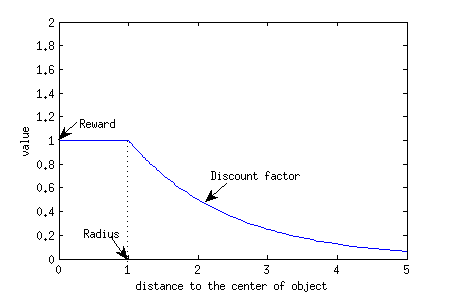
\includegraphics[width=0.8\textwidth]{figs/modularQ}
\caption{A modular value function configured by reward, discount factor and
radius of the object.}
\label{fig:modularQ}
\end{figure}

We made the same assumption as modular RL that the global Q function is the sum
of modular Q functions. We redefine the modular Q functions here to accept the 
parameter $p$\DIFaddbegin \DIFadd{, as follows}\DIFaddend .
\begin{equation}
Q(s_t,a_t) = \sum_{n=1}^{N} Q^{(n)}(s_t^{(n)},a_t,p^{(n)})
\end{equation}

We didn't make any assumption on the prior distribution of the parameters, so
the objective is to maximize the sample likelihood. We assume that the expert
uses a softmax function in action selection. The objective function is

\begin{equation}
\label{eq:irl}
\max_{p} \prod_t \frac{e^{\eta Q(s_t, a_t)}}{\sum_b e^{\eta Q(s_t,
b)}}
\end{equation}, where \DIFdelbegin \DIFdel{$a^{(t)}$ }\DIFdelend \DIFaddbegin \DIFadd{$a_t$ }\DIFaddend is the action selected by the expert, and $b$
iterates over other possible actions. This is equivalent to maximizing the log
of this function.
\begin{align}
&\max_{p} \log \prod_t \DIFdelbegin \DIFdel{\frac{e^{\eta Q(s_t, a_t)}}{\sum_b e^{\eta Q(s_t,
b}}}\DIFdelend \DIFaddbegin \DIFadd{\frac{e^{\eta Q(s_t, a_t)}}{\sum_b e^{\eta Q(s_t,
b)}}}\DIFaddend \\
=&\max_{p} \sum_t (\eta Q(s_t, a_t) \DIFdelbegin \DIFdel{) }\DIFdelend - \log \sum_b e^{\eta Q(s_t, b)}\DIFaddbegin \DIFadd{)
}\DIFaddend \label{eq:irllog}\\
=&\max_{p} \sum_t (\eta \sum_i Q\DIFdelbegin \DIFdel{_i}\DIFdelend \DIFaddbegin \DIFadd{^{(i)}}\DIFaddend (s_t^{(i)}, a_t, p^{(i)}) - \log \sum_b e\DIFdelbegin \DIFdel{^{\eta \sum_i
Q_i(s_t^{(i)}, b, p^{(i)})}}\DIFdelend \DIFaddbegin \DIFadd{^{\eta \sum_i
Q^{(i)}(s_t^{(i)}, b, p^{(i)})}}\DIFaddend )
\end{align}

In some cases, we may want to add a regularization factor. In general, we
modify the objective function to be as follows.

\begin{equation}
\label{eq:irl}
\max_{p} \sum_t (\eta \sum_i Q\DIFdelbegin \DIFdel{_i}\DIFdelend \DIFaddbegin \DIFadd{^{(i)}}\DIFaddend (s_t^{(i)}, a_t, p^{(i)}) - \log \sum_b e\DIFdelbegin \DIFdel{^{\eta \sum_i
Q_i(s_t^{(i)}, b, p^{(i)})}}\DIFdelend \DIFaddbegin \DIFadd{^{\eta \sum_i
Q^{(i)}(s_t^{(i)}, b, p^{(i)})}}\DIFaddend )
- \lambda ||p'||_1
\end{equation},
where $p'$ is a vector such that $p'_i = p_i\ ||\ 0$. $\lambda$ is the
regularization parameter. So we can regularize some supports of $p$. For
example, in a driving task, human subjects can only pay attention to \DIFaddbegin \DIFadd{a }\DIFaddend certain
number of modules. To immitate such behavior, we may force the reward vector to
be sparse. In this way, we can define many possible modules and feed them into the
algorithm, the algorithm will determine which are the non-significant modules,
which would have rewards of 0.

We notice that this function may not be convex. So we use a nonconvex optimization
solver. Concretely, we use evolution strategy with covariance matrix adaptation (CMA-ES)
\cite{hansen2003reducing} for the experiments in the evaluation chapter.


\chapter{Literature Review}
\label{chp:lr}
\section{Task Decomposition}

Modularization is one approach to reduce the dimension of the state space. In
this section, we will discuss some major approaches of MDP decomposition as
solutions to the curse of dimensionality, and analyze their similarity and
difference compared to the modular approach. We will discuss a hierarchical
approach and a layered approach.

Some complex tasks have explicit phases. Take the taxi domain for example
(Figure~\ref{fig:taxi}). The taxi driver picks up a passenger from a location,
and drives and drops him at a different location. This task requires some shared
low-level skills.

\begin{figure}[h]
\centering
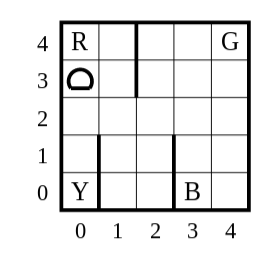
\includegraphics[width=0.3\textwidth]{taxi.png}
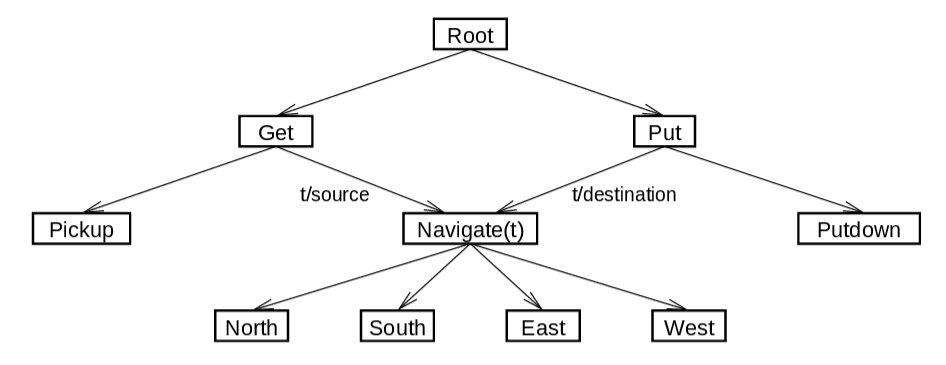
\includegraphics[width=0.6\textwidth]{maxq.png}
\caption{(Left) Taxi domain. (Right) A decomposition of the task.}
\label{fig:taxi}
\end{figure}

This is generally known as hierarchical reinforcement learning (hierarchical RL)
\cite{dietterich2000hierarchical}.
We assume that there is a known structure of the task, and the
learning is decomposed hierarchically. At a higher level, an action can be
which lower level task to execute. For example, in the Get task, the two actions
available would be Pickup and Navigate. At the bottom level, primary actions are
accessible.

A similar approach is skill chaining \cite{konidaris2009skill}, which can
be seen as a hierarchical RL approach. Figure~\ref{fig:skills} shows
an example that a robot navigates in a domain with obstacles. The red circle is
the goal. The robot starts from the left-bottom corner. It has several trained
skills, represented by different colors. The robot learns which skill to use,
and when to terminate and switch to another skill.

\begin{figure}[h]
\centering
\includegraphics[width=0.5\textwidth]{skills}
\caption{Skill chaining in robot motion.}
\label{fig:skills}
\end{figure}

Hierarchical reinforcement learning is different from modular reinforcement
learning in a way that the former approach doesn't involve concurrent modules
(or subtasks, skills, depending on the context).
For example, the Pickup module doesn't run parallel with Navigate module.
Therefore, there is no compromise in policies proposed by different modules.

Apart from hierarchical RL, layered learning is another approach to decompose a
complex task \cite{stone2000layered}. This is a general learning method that may
not \DIFaddbegin \DIFadd{be }\DIFaddend restricted to reinforcement learning. Similar to hierarchical learning, it
also assumes a hierarchy of the task. A module has some parameters. The
optimization \DIFdelbegin \DIFdel{startes }\DIFdelend \DIFaddbegin \DIFadd{starts }\DIFaddend from the bottom layer. When the \DIFdelbegin \DIFdel{parametres }\DIFdelend \DIFaddbegin \DIFadd{parameters }\DIFaddend in modules in
the same layer are optimized, the optimization for the upper layer starts. A
module will use the modules in the lower layers.

One example is learning in robot soccer. In Figure~\ref{fig:soccer}, each block
is an module. The number in the parenthesis is the number of parameters involved
in each module. The arrows indicate the dependency relations between modules.
Training starts from the bottom layer, then \DIFdelbegin \DIFdel{propagate }\DIFdelend \DIFaddbegin \DIFadd{propagates }\DIFaddend upwards to higher level
layers.
A recent work in layered learning makes some parameters in lower level modules
available to change in the process of training of a higher level module
\cite{macalpine2015ut}. This is the same idea as parameterizing modules in
modular inverse reinforcement learning. 

\begin{figure}[h]
\centering
\includegraphics[width=\textwidth]{layered}
\caption{Layered learning in robot soccer. \cite{macalpine2015ut}}
\label{fig:soccer}
\end{figure}

Layered learning is similar to modular reinforcement learning, as the modules are
run in parallel. However different modules correspond to different controllers
or agents. They need to compromise to contribute to a higher level module, but
not sharing a uniform output interface.

\section{Inverse Reinforcement Learning}

We introduced basic concepts of inverse reinforcement learning in the last
chapter. In this section, we discuss some advances in IRL and compare them with
our methods.

The original IRL algorithm is formulated by
\cite{abbeel2004apprenticeship,ng2000algorithms}. A popular following work is
Bayesian inverse reinforcement learning (Bayesian IRL) \cite{ramachandran2007bayesian}.
It is motivated by the
observation that rewards are not completely arbitrary. We can reasonably assume
some prior knowledge of the rewards. Bayesian IRL assumes that the rewards are
drawn from a prior distribution. 
For example, in most of the problems, rewards are generally sparse. So the
reward of a state is very likely to be 0. A Gaussian or Laplacian prior can be
applied.  In planning problems, on the contrary, rewards are generally small but
positive for most of the states. Then a Beta prior can be applied.
Concretely, according to the Bayes rule,
$$P(R|O) = \frac{P(O|R)P(R)}{P(O)}$$
, where $O$ is the observed data, $R$ is the reward vector. Bayesian IRL assumes
$P(R)$ to be non-uniform.

Other recent developments in Bayesian IRL include
\cite{choi2011map,choi2012nonparametric,dimitrakakis2012bayesian}.
\cite{choi2011map} uses MAP inference to solve the Bayesian IRL problem.
\cite{choi2012nonparametric,dimitrakakis2012bayesian} tackle the problem of
recovering rewards in domains with multiple tasks or multiple rewards. 


\chapter{Evaluations and Applications}
\label{chp:eval}
\section{Preliminary Evaluation}

In this section, we evaluate the modular inverse reinforcement learning
algorithm in a navigation domain. We have access to the ground truth of the
parameters of all the modules. This helps us to empirically verify the
correctness and efficiency of the algorithm.

\subsection{Sanity Check}

We test the algorithm in a grid world domain with 2 modules. Each has several
objects. Different modules have different parameters, including rewards and discount
factors. The objects of same module share the same parameters. The agent only
considers the closest object in each module as its state space. It can
obtain the corresponding reward when reaching in a grid with an object.

According to the definition of the global \DIFaddbegin \DIFadd{Q }\DIFaddend function, $Q(s, a) = Q^{(1)}(s^{(1)},
a) + Q^{(2)}(s^{(2)}, a)$. Where $s^{(1)}, s^{(2)}$ are the distances to the
closest objects in each module.

We show the heatmaps of the value functions of some sample domains with one
 in Figure~\ref{fig:sanity}. This helps us to visualize the effect of different
 parameters with same configuration of objects. For simplicity, we only show the
 case with one object in each module.

\begin{figure}
\centering
\begin{subfigure}{0.45\textwidth}
\includegraphics[width=\textwidth]{figs/continuous_world_values0}
\caption{$r_1=1, r_2=1, \gamma_1=.9, \gamma_2=.9$}
\end{subfigure}

\begin{subfigure}{0.45\textwidth}
\includegraphics[width=\textwidth]{figs/continuous_world_values1}
\caption{$r_1=1, r_2=1, \gamma_1=.9, \gamma_2=.1$}
\end{subfigure}

\begin{subfigure}{0.45\textwidth}
\includegraphics[width=\textwidth]{figs/continuous_world_values2}
\caption{$r_1=1, r_2=-1, \gamma_1=.9, \gamma_2=.9$}
\end{subfigure}
\caption{Heatmap of value function in a navigation domain. The red color
indicates higher value. There are 2 modular
objects. Object \#1 is in upper-left and Object \#2 is in lower-right.  Rewards
and discount factors are specified for these two objects (as $r_1, r_2, \gamma_1,
\gamma_2$).}
\label{fig:sanity}
\end{figure}

We use the modular Q \DIFdelbegin \DIFdel{function }\DIFdelend \DIFaddbegin \DIFadd{functions }\DIFaddend and observed policies on all the states as input
to our modular IRL algorithm, and run our algorithm to recover the underlying
parameters for both modules. The dimension of the gridworld is 20$\times$20.
There are 5 objects in each module. The results are shown in Table~\ref{tbl:sanity}.
We can observe that in some cases the discount factors are not recovered
correctly. This happens when a range of parameters can explain the same observed policy.

\begin{table}[h]
\centering
\begin{tabular}{l | l l l l}
\hline
 & $r_1$ & $r_2$ & $\gamma_1$ & $\gamma_2$\\
\hline
Task 1, Ground Truth & 1 & 1 & 0.9 & 0.9 \\
Task 1, Recovered & 1.0 & 1.0 & 0.87 & 0.91 \\
\hline
Task 2, Ground Truth & 1 & 1 & 0.9 & 0.1 \\
Task 2, Recovered & 1.0 & 1.0 & 0.89 & 0.01 \\
\hline
Task 3, Ground Truth & 1 & -1 & 0.9 & 0.9 \\
Task 3, Recovered & 1.0 & -1.0 & 0.86 & 0.54 \\
\hline
\end{tabular}
\caption{Ground truth and recovered parameters in three gridworld domains.}
\label{tbl:sanity}
\end{table}

\subsection{Comparison with Non-Modular Inverse Reinforcement Learning}

We compare our algorithm with non-modular Bayesian inverse reinforcement
learning \cite{ramachandran2007bayesian} to demonstrate the sample efficiency
advantage of the modular approach.
In Bayesian IRL, we assume a prior distribution of the reward function. We use a
Laplacian prior in Bayesian IRL since the rewards are sparse. Because
traditional IRL algorithms can only recover rewards, we make our modular IRL
algorithm to recover the same.

In Figure~\ref{fig:mVSb}, we report the sample
efficiency of modular IRL versus Bayesian IRL. There are 4 modules and
each has 4 objects. We run both algorithms with different number of samples
(state-policy pairs). We then compare the policies generated using the learned
rewards. Policy agreement is defined as the proportion of the states that have
the same policies as the ground truth. We use the metric of policy agreement in
our comparison since the outputs of these two algorithms can not be directly
compared. Our observation is that modular IRL obtained nearly 100\% policy
agreement with far fewer samples compared to the non-modular approach.

\begin{figure}[h]
\centering
\includegraphics[width=0.6\textwidth]{figs/grid_modular_vs_bayes}
\caption{Modular IRL vs Bayesian IRL on sample efficiency, measured by policy agreement.}
\label{fig:mVSb}
\end{figure}


\section{Human Experiment Results}
% Shun

In this section, we report results from the human virtual navigation experiment. We hypothesize that behavior data can be modeled by our maximum likelihood modular IRL framework and test against baseline models. Figure~\ref{fig:avatar} shows the experimental setup. The human subjects wore a binocular head-mounted
display. The subjects' eye, head, and body motion were tracked while walking through a virtual room. The subjects were asked to collect the targets (blue spheres) by intercepting them, follow the path (the gray line), and avoid the obstacles (red cubes). Thus this domain has three module classes: following the path, collecting targets, and avoiding obstacles. This general paradigm has been used to evaluate modular IRL algorithms \cite{rothkopf2013modular} and to study human navigation and gaze behavior \cite{Tong2014}.

\begin{figure}
\centering
\includegraphics[height=4cm]{figs/human.jpg}
\includegraphics[height=5cm]{figs/env.png}
\caption{The second test domain. (Left) A human subject wears a head mounted display (HMD) and trackers
for eyes, head, and body.  (Right) The virtual environment as seen through
the HMD.  The red cubes are obstacles and the blue spheres are targets.
There is also a gray path on the ground which the human subject were told to follow.}
\label{fig:avatar}
\end{figure}

We gave subjects four types of task instructions, resulting in 4 experimental conditions:
\begin{itemize}
\item {\bf Task 1}: Follow the path only and ignore objects 
\item {\bf Task 2}: Follow the path and avoid the obstacles  
\item {\bf Task 3}: Follow the path and collect targets 
\item {\bf Task 4}: Follow the path, collect targets, and avoid obstacles.  
\end{itemize}
Subjects received auditory feedback when running into obstacles or targets, but only when the objects were task relevant. Here we examined data collected from 4 human subjects. Each subject walked through the environment 8 times for each experimental condition, resulting in 32 experimental trials. In each trial the configuration of objects was different. 

\begin{figure}
\centering
\begin{subfigure}[b]{0.48\textwidth}
\includegraphics[width=\textwidth]{figs/task_1.png}
\caption{Path only\\
Rewards: [.035, -.017, {\bf .948}]\\
Discount factors: [.892, 0.181, .900]}
\end{subfigure}
\begin{subfigure}[b]{0.48\textwidth}
\includegraphics[width=\textwidth]{figs/task_2.png}
\caption{Path + Obstacle \\
Rewards: [.000, {\bf -.227}, {\bf .773}]\\
Discount factors: [.900, .134, .618]}
\end{subfigure}
\begin{subfigure}[b]{0.48\textwidth}
\includegraphics[width=\textwidth]{figs/task_3.png}
\caption{Path + Target\\
Rewards: [{\bf .395}, -.098, {\bf .506}]\\
Discount factors: [.189, .100, .407]}
\end{subfigure}
\begin{subfigure}[b]{0.48\textwidth}
\includegraphics[width=\textwidth]{figs/task_4.png}
\caption{Path + Target + Obstacle \\
Rewards: [{\bf .312}, {\bf -.180}, {\bf .508}]\\
Discount factors: [.148, .100, .570]}
\end{subfigure}
\caption{The trajectories of the human subjects and the agent in four conditions. Targets are
blue and obstacles are red. The black lines are trajectories of human subjects,
and the green lines are trajectories of the RL agent trained using the recovered
rewards and discount factors. The rewards and discount factors are shown in [Target,
Obstacle, Path] format. The rewards are normalized to sum to 1. The rewards that
correspond to task instructions are bold.}
\label{fig:exp}
\end{figure}

We use Equation \ref{eq:irllog} as our objective function to recover $r$ and $\gamma$. Our agent uses the distance and angle to the module instances as state information. We constrain the action set of the agent to be human-like; it takes discrete forward actions, ranging from turning left 90 degrees to turning right 90 degrees. 

The results are shown in Figure \ref{fig:exp}. It is clear that the estimated $r$ agreed with our task instructions. We then trained an agent with the recovered $r$ and $\gamma$, and let the agent navigate in the same environment. The resulting agent trajectories (shown in green) are compared with human trajectories (shown in black) in Figure~\ref{fig:exp}. 

\begin{table}
\centering
\begin{tabular}{l | l l l}
\hline
Task & Agent  & \shortstack{Angular Diff.} & Log Likelihood  \\
\hline
\multirow{3}{*}{Path only}
& Modular  & 25.820  & -3914.196 \\
& Reflex  & 35.600  & -3916.157 \\
& Random  & 55.219  & -3926.847 \\
\hline
\multirow{3}{*}{Obstacle + Path}
& Modular  & 33.988  & -4950.079 \\
& Reflex  & 63.884  & -4985.290 \\
& Random  & 55.717  & -4989.314 \\
\hline
\multirow{3}{*}{Target + Path}
& Modular  & 33.918  & -4855.531 \\
& Reflex  & 37.176  & -4838.832 \\
& Random  & 55.012  & -4909.531 \\
\hline
\multirow{3}{*}{All}
& Modular  & 39.034  & -6175.692 \\
& Reflex  & 45.307  & -6164.702 \\
& Random  & 55.961  & -6221.075 \\
\hline
\end{tabular}
\caption{Evaluation on the modular agent's performance compared with two
baseline agents.}
\label{tbl:humanStat}
\end{table}

\begin{figure}
\centering
\begin{subfigure}[b]{0.45\textwidth}
\includegraphics[width=\textwidth]{figs/contact1.png}
\DIFdelbeginFL %DIFDELCMD < \caption{%
{%DIFAUXCMD
\DIFdelFL{Path module only. }}
%DIFAUXCMD
\DIFdelendFL \end{subfigure}
\begin{subfigure}[b]{0.45\textwidth}
\includegraphics[width=\textwidth]{figs/contact2.png}
\DIFdelbeginFL %DIFDELCMD < \caption{%
{%DIFAUXCMD
\DIFdelFL{Obstacle + Path. }}
%DIFAUXCMD
\DIFdelendFL \end{subfigure}
\begin{subfigure}[b]{0.45\textwidth}
\includegraphics[width=\textwidth]{figs/contact3.png}
\DIFdelbeginFL %DIFDELCMD < \caption{%
{%DIFAUXCMD
\DIFdelFL{Target + Path. }}
%DIFAUXCMD
\DIFdelendFL \end{subfigure}
\begin{subfigure}[b]{0.45\textwidth}
\includegraphics[width=\textwidth]{figs/contact4.png}
\DIFdelbeginFL %DIFDELCMD < \caption{%
{%DIFAUXCMD
\DIFdelFL{Target + Obstacle + Path. }}
%DIFAUXCMD
\DIFdelendFL \end{subfigure}
\caption{Number of targets hit and number of obstacles hit of the human subjects 
and the agent.}
\label{fig:stats}
\end{figure}

We compared the performance of our agent with two baseline agents, shown in
Table~\ref{tbl:humanStat}. The {\em Random Agent} takes an action randomly
without considering state information. The {\em Reflex Agent} greedily chases the nearest target or avoids the nearest obstacle, depending on which is closer. We considered two evaluation metrics. The first is the {\em angular difference} of
the policies between the human subjects and the
agent. For every state-policy pair in the human data, we
compared the action the human took to the action our agent would select in the same state, taking the difference in angle between the chosen actions. The second metric is the {\em logarithm of the likelihood}, which is the
probability that the human data is generated by the learned
parameters. The results are shown in Table \ref{tbl:humanStat}. The modular agent is more similar to the human subjects than the other two agents in terms of angular difference. However, in the last two tasks, it has similar performance with the reflex agent using the likelihood metric.

Figure~\ref{fig:stats} evaluates the performance by showing the number of
targets hit and number of obstacles hit.  The number of targets hit should be
large, and the number of obstacles hit should be small, when the corresponding
module is active.  We can observe that humans still do better than the agent in
these tasks.  Nevertheless, the agent performance is quite similar to that of
the human subjects.

\begin{figure}
\centering
\DIFdelbeginFL %DIFDELCMD < \begin{subfigure}[b]{0.45\textwidth}
%DIFDELCMD < %%%
\DIFdelendFL \DIFaddbeginFL \begin{subfigure}[b]{0.49\textwidth}
\DIFaddendFL \includegraphics[width=\textwidth]{figs/objValuesTask1.png}
\caption{Path following only.}
\end{subfigure}
\DIFdelbeginFL %DIFDELCMD < \begin{subfigure}[b]{0.45\textwidth}
%DIFDELCMD < %%%
\DIFdelendFL \DIFaddbeginFL \begin{subfigure}[b]{0.49\textwidth}
\DIFaddendFL \includegraphics[width=\textwidth]{figs/objValuesTask2.png}
\caption{Obstacle + Path. }
\end{subfigure}
\DIFdelbeginFL %DIFDELCMD < \begin{subfigure}[b]{0.45\textwidth}
%DIFDELCMD < %%%
\DIFdelendFL \DIFaddbeginFL \begin{subfigure}[b]{0.49\textwidth}
\DIFaddendFL \includegraphics[width=\textwidth]{figs/objValuesTask3.png}
\caption{Target + Path. }
\end{subfigure}
\DIFdelbeginFL %DIFDELCMD < \begin{subfigure}[b]{0.45\textwidth}
%DIFDELCMD < %%%
\DIFdelendFL \DIFaddbeginFL \begin{subfigure}[b]{0.49\textwidth}
\DIFaddendFL \includegraphics[width=\textwidth]{figs/objValuesTask4.png}
\caption{Target + Obstacle + Path. }
\end{subfigure}
\caption{Heatmaps of the $\log$ of the values of Equation~\ref{eq:irllog} for
different rewards for the four tasks, respectively. The white zones indicate
higher probabilities. The weights of all three modules sum to 1, so we only show
the weights on the target and the obstacle modules.
}
\label{fig:heatmap}
\end{figure}

It is of interest to see the objective function value of different rewards. To
present the rewards, we use the term \textit{weights} to represent the
normalized rewards which sum to 1. For example, the reward vector of (1, -1, 2)
corresponds to the weight vector (0.25, 0.25, 0.5). It would be difficult to
visualize the whole solution space because of the dimensionality. We report the
results for different rewards, but with the discount factors fixed to be the solved optimal
values.
This is shown in Figure~\ref{fig:heatmap}. The colors represent the $\log$ of values of
Equation~\ref{eq:irllog} for different weights. The white color represents higher
probability. We can observe the centroids of white zones move for different
tasks. It stays at the origin in Task 1, so neither the target module nor the
obstacle module is active. It moves away from the origin when a module is
active.  From the heatmaps, we find that optima exist for these tasks and match
our solutions. We also find out that with the discount factors fixed, the
solution space is convex. This can be verified in Equation~\ref{eq:irllog}.

\DIFdelbegin \DIFdel{We then look at }\DIFdelend \DIFaddbegin \DIFadd{It is also of interest to see whether different human subjects have different
parameters for the same task, and whether same human subjects use the same
parameters for all the trials.
We look at the }\DIFaddend differences of $r$ and $\gamma$ within subjects and between
subjects in Task 4. The results are shown in Figure~\ref{fig:humanIndividuals}.
Within-subjects consistency indicates if the same subject has similar $r$ and
$\gamma$ in different trials of Task 4, measured by the confidence interval (the
errorbar). Between-subjects consistency indicates if different subjects have
similar $r$ and $\gamma$ on average in Task 4, measured by the mean value (the
height of bar).

First, we observe that both rewards and discounters are similar for each module
for all the human subjects. For example, the discount factors for the path
module are generally large, which means that the value is still large even not
strictly following the path. This intuitively matches human's behavior on path
following. On the contrary, the discount factors for the target module are
small, because people want to make sure that they reach the target and get the
positive reward. The value is small even slightly off the target.
For $r$, an interesting observation is that subjects may have
different rewards for modules, even though they are given the same task
instruction. Subject \#3 is different than the other subjects, as he/she clearly
weighted collecting targets less and following path more.

\begin{figure}
\centering
\includegraphics[width=0.45\textwidth]{figs/human_individuals_weights}
\includegraphics[width=0.45\textwidth]{figs/human_individuals_discounters}
\caption{The weights (normalized rewards, on the left) and discount factors (on
the right) of different human subjects in Task 4. The error bars are 95\%
confidence intervals.}
\label{fig:humanIndividuals}
\end{figure}



\chapter{Conclusion}
\label{chp:conclude}
In this thesis, we followed an earlier work on modular inverse reinforcement
learning. We proposed a new modular inverse reinforcement
learning algorithm, and applied it to collected human subjects' data to analyze
their behavior.
The experimental results show that modular reinforcement learning can explain
human's navigation behavior. By our evaluation metrics, this method is better
than \DIFaddbegin \DIFadd{the }\DIFaddend other baseline assumptions.

We have discussed in the literature review that modular approach is just one way to combine multiple
sub-MDPs. There are other assumptions that can be evaluated in the future work.
For example, scheduling between
different modules, with only one active at one time. This is close to the skill
switching method \cite{konidaris2009skill}. However, we adopt the
weighted sum approach because this is more reasonable for human behavior. When a
human tries to collect targets while avoiding obstacles, these two modules are
expected to be both active. A scheduling approach may yield frequent oscillation
between these two modules.

Static combination of modules throughout a task is another assumption that
should be removed in the future work. Parameters may be dynamic and different from
state to state.  However, with such an assumption we need to learn a mapping
from state to parameters. In this case, the curse of dimensionality still exists,
and inverse learning would be difficult.

So far, we only used the motion data of human subjects. There is also gaze data
collected but not used. Gazes are the points that human subjects are looking at
at a time step, which indicate humans' attention. This is actually a useful
information on how human combines different modules. When a human is paying
attention to a module, it is reasonable to assume that his action would be
affected mainly by this module.

In sum, we show in this thesis that modular reinforcement learning is a
promising explanation for human's navigation behavior. It is of interest to see
its analysis on different humans' behavior, and using the recovered parameters
for a learning agent to tackle similar tasks.


%%%%%%%%%%%%%%%%%%%%%%%%%%%%%%%%%%%%%%%%%%%%%%%%%%%%%%%%%%%%%%%%%%%%%%
% Appendix/Appendices                                                %
%%%%%%%%%%%%%%%%%%%%%%%%%%%%%%%%%%%%%%%%%%%%%%%%%%%%%%%%%%%%%%%%%%%%%%
%
% If you have only one appendix, use the command \appendix instead
% of \appendices.
%
\appendices
\index{Appendices@\emph{Appendices}}%

%%%%%%%%%%%%%%%%%%%%%%%%%%%%%%%%%%%%%%%%%%%%%%%%%%%%%%%%%%%%%%%%%%%%%%
% Generate the bibliography.					     %
%%%%%%%%%%%%%%%%%%%%%%%%%%%%%%%%%%%%%%%%%%%%%%%%%%%%%%%%%%%%%%%%%%%%%%
%								     %
% NOTE: For master's theses and reports, NOTHING is permitted to     %
%	come between the bibliography and the vita. The command      %
%	to generate the index (if used) MUST be moved to before      %
%	this section.						     %
%								     %
%\nocite{*}      % This command causes all items in the 		     %
                % bibliographic database to be added to 	     %
                % the bibliography, even if they are not 	     %
                % explicitly cited in the text. 		     %
		%						     %
\bibliographystyle{plain}  % Here the bibliography 		     %
\bibliography{diss,nips15/paper,RLLiterature/report}        % is inserted.			     %
\index{Bibliography@\emph{Bibliography}}%			     %
%%%%%%%%%%%%%%%%%%%%%%%%%%%%%%%%%%%%%%%%%%%%%%%%%%%%%%%%%%%%%%%%%%%%%%


%%%%%%%%%%%%%%%%%%%%%%%%%%%%%%%%%%%%%%%%%%%%%%%%%%%%%%%%%%%%%%%%%%%%%%
% Generate the index.						     %
%%%%%%%%%%%%%%%%%%%%%%%%%%%%%%%%%%%%%%%%%%%%%%%%%%%%%%%%%%%%%%%%%%%%%%
%								     %
% NOTE: For master's theses and reports, NOTHING is permitted to     %
%	come between the bibliography and the vita. This section     %
%	to generate the index (if used) MUST be moved to before      %
%	the bibliography section.				     %
%								     %
\printindex%    % Include the index here. Comment out this line      %
%		% with a percent sign if you do not want an index.   %
%%%%%%%%%%%%%%%%%%%%%%%%%%%%%%%%%%%%%%%%%%%%%%%%%%%%%%%%%%%%%%%%%%%%%%


%%%%%%%%%%%%%%%%%%%%%%%%%%%%%%%%%%%%%%%%%%%%%%%%%%%%%%%%%%%%%%%%%%%%%%
% Vita page.							     %
%%%%%%%%%%%%%%%%%%%%%%%%%%%%%%%%%%%%%%%%%%%%%%%%%%%%%%%%%%%%%%%%%%%%%%

%\begin{vita}
%\end{vita}

\end{document}
